% !TEX encoding = UTF-8
% !TEX TS-program = pdflatex
% !TEX root = ../tesi.tex

%**************************************************************
\chapter{Analisi dei requisiti}
\label{cap:analisi_dei_requisiti}
%**************************************************************
In questo capitolo verranno esposti i casi d'uso e i requisiti del modulo \gls{ITF} oggetto del lavoro di stage.\\
Si procede con la descrizione dello stato del sistema, gli attori che vi partecipano, le pre-condizioni, le post-condizioni e gli scenari.\\
I casi d'uso principali sono associati ad un diagramma \gls{uml} 2.0 che riporta lo stesso codice identificativo e titolo del caso d'uso al quale si riferisce.

%**************************************************************
\section{Dominio}
\subsection{Caratteristiche degli attori}
L'interazione con il modulo \gls{ITF} coinvolge essenzialmente tre tipologie diverse di attori:
\begin{itemize}
	\item l'identity wallet;
	\item un ente certificatore;
	\item un service provider.
\end{itemize}

\subsubsection{Identity Wallet}
Questa componente del sistema ha il compito di generare, mantenere e presentare l'identità digitale dell'utente. A sua volta, l'\textit{Identity Wallet} interagisce con il sistema \gls{ITF} nel momento in cui un utente esegue una richiesta di accesso verso un \textit{service provider} il quale richiede l'autenticazione e la conferma delle credenziali insieme alla verifica di attributi specifici necessari per erogare i suoi servizi.\\
Il sistema \gls{monokee}, una volta che l'utente richiede l'accesso ad un \textit{service provider}, reindirizza la richiesta di accesso all'\gls{ITF}.
\subsubsection{Ente Certificatore (Trusted Third Party)}
La seconda tipologia di attori che interagiscono con il sistema da realizzare sono i \textit{Trusted Third Party}.\\
Questi, chiamati enti certificatori, hanno il compito di certificare le informazioni che sono presenti all'interno dell'\gls{ITF} in modo che, ogni volta che vengono richieste per poter accedere ad un \textit{service provider}, le informazioni che il sistema fornisce per l'autenticazione e/o l'erogazione di servizi siano verificate da un ente esterno che garantisce la loro veridicità.
\subsubsection{Service Provider}
La terza e ultima tipologia di attori che partecipano al sistema sono i \textit{service provider}.
Questi interagiscono con l'\gls{ITF} durante la fase di verifica delle informazioni. Questi devono autenticare gli utenti tramite le loro credenziali e autorizzare l'erogazione di servizi dopo la verifica degli attributi.
%**************************************************************
\subsection{Overview del sistema}
Una rappresentazione delle funzionalità che deve implementare il modulo \gls{ITF} può essere ripresa in Figura \ref{fig:moduloITF}.\\\\
Il prodotto finale prevede l'interazione delle tre tipologie di attori allo scopo di garantire:
\begin{itemize}
	\item l'accesso sicuro al \textit{service provider} desiderato;
	\item l'erogazione dei servizi offerti dal \textit{service provider} in modo controllato.
\end{itemize}
Questo viene garantito dall'\gls{ITF} e dalla tecnologia \textit{Blockchain} che ne è alla base.\\
Di seguito viene descritto il flusso di chiamate che intercorrono affinchè un utente possa accedere ad uno o più servizi di sua scelta.\\\\
Quando un utente richiede dei servizi, da parte di un \textit{service provider}, il sistema viene interrogato e inizia lo scambio di informazioni che coinvolge l'\textit{identity wallet}, gli enti certificatori ed il \textit{service provider}.\\
Ogni qual volta un utente richiede l'accesso a dei servizi di un determinato \textit{service provider}, \gls{monokee} reindirizza la richiesta d'accesso all'\textit{identity wallet} che, a sua volta, invia la richiesta di accesso all'\gls{ITF} passandogli un identificativo dell'utente che ha fatto la richiesta di accesso insieme alle informazioni che il \textit{service provider} necessita per poter permettere l'erogazione dei suoi servizi.\\
Nell'\gls{ITF} viene eseguita una ricerca nella rete \textit{Blockchain} sottostante in modo da verificare se le informazioni richieste dal \textit{service provider} siano effettivamente associate all'utente. Se il riscontro è positivo, il \textit{service provider} permette l'accesso all'utente altrimenti gli viene negato.\\\\
La seconda tipologia di attori che partecipano al sistema, gli enti certificatori, entrano in gioco durante la fase di registrazione di un nuovo utente o quando un amministratore di dominio associa degli attributi alle identità digitali dei suoi utenti.
Gli enti certificatori hanno il compito di verificare e certificare che, le asserzioni o gli attributi, di una particolare identità, siano conformi alle informazioni associate a quell'utente.\\
Questo ruolo è di fondamentale importanza all'interno del sistema che si sta sviluppando in quanto, essendo l'\gls{ITF} basata su una \textit{Blockchain}, tutte le informazioni che popolano la rete sono immutabili e, quindi, prima di essere definitivamente inserite in un blocco, devono essere verificate e approvate, dagli enti certificatori, tramite gli algoritmi di consenso.\\\\
La terza tipologia di attori, i \textit{service providers}, interagiscono con il sistema durante la verifica delle informazioni dell'identità dell'utente.\\
Questi, dopo che l'\textit{identity wallet} gli ha passato i record contenenti la chiave pubblica e il riferimento alla locazione del record cifrato nell'\gls{ITF}, iniziano il  controllo delle informazioni.\\
Il controllo viene fatto andando prima a calcolare l'\textit{hash crittografico} della chiave pubblica pervenuta dall'\textit{identity wallet} e poi andando a confrontare il risultato ottenuto con quello presente nell'\gls{ITF} recuperato grazie al riferimento alla sua locazione nella rete Blockchain.
In questa fase, il \textit{service provider} verifica i record contenente l'identità e qualsiasi altra credenziale per autenticare l'utente e verifica anche gli attributi necessari per autorizzare l'utente ad utilizzare i suoi servizi.
\section{Casi d'uso}
\subsection{Classificazione dei casi d'uso}
Ogni caso d'uso è classificato secondo la seguente convienzione:\\\\
\centerline{UC[codicePadre]\_[codiceFiglio]}\\\\
In cui i due codici rappresentano:
\begin{itemize}
	\item \textbf{codicePadre} - identifica univocamente il caso d'uso;
	\item \textbf{codiceFiglio} - identifica univocamente i sotto casi d'uso appartenenti ad un determinato "codicePadre".
\end{itemize}

\subsection{Descrizione dei casi d'uso}
Ogni caso d'uso viene descritto dalla seguente struttura:
\begin{itemize}
	\item \textbf{Descrizione} - Breve descrizione del caso d'uso che si sta modellando;
	\item \textbf{Attori Principali} - Indica l'attore principale del caso d'uso. In tutto il contesto dell'applicazione, gli attori saranno classificati come:
	\begin{itemize}
		\item Identity Wallet;
		\item Trusted Third Party (ente certificatore);
		\item Service Provider.
	\end{itemize}
	\item \textbf{Attori Secondari} - Indica l'attore che aiuta l'attore principale a realizzare quanto descritto dal caso d'uso;
	\item \textbf{Pre-Condizioni} - Specifica la condizione del sistema prima del verificarsi degli eventi descritti dal caso d'uso;
	\item \textbf{Post-Condizioni} - Specifica le condizioni del sistema dopo il verificarsi degli eventi descritti dal caso d'uso;
	\item \textbf{Scenario Principale} - Rappresenta il flusso principale degli eventi ovvero il caso in cui tutto funzioni come deve;
	\item \textbf{Estensioni} - Rappresenta il flusso secondario degli eventi nel caso in cui si verifichino degli errori nel flusso principale.
\end{itemize}
\newpage
\subsection{Caso d'uso UC1: Registrazione}
\begin{figure}[!h]
	\centering
	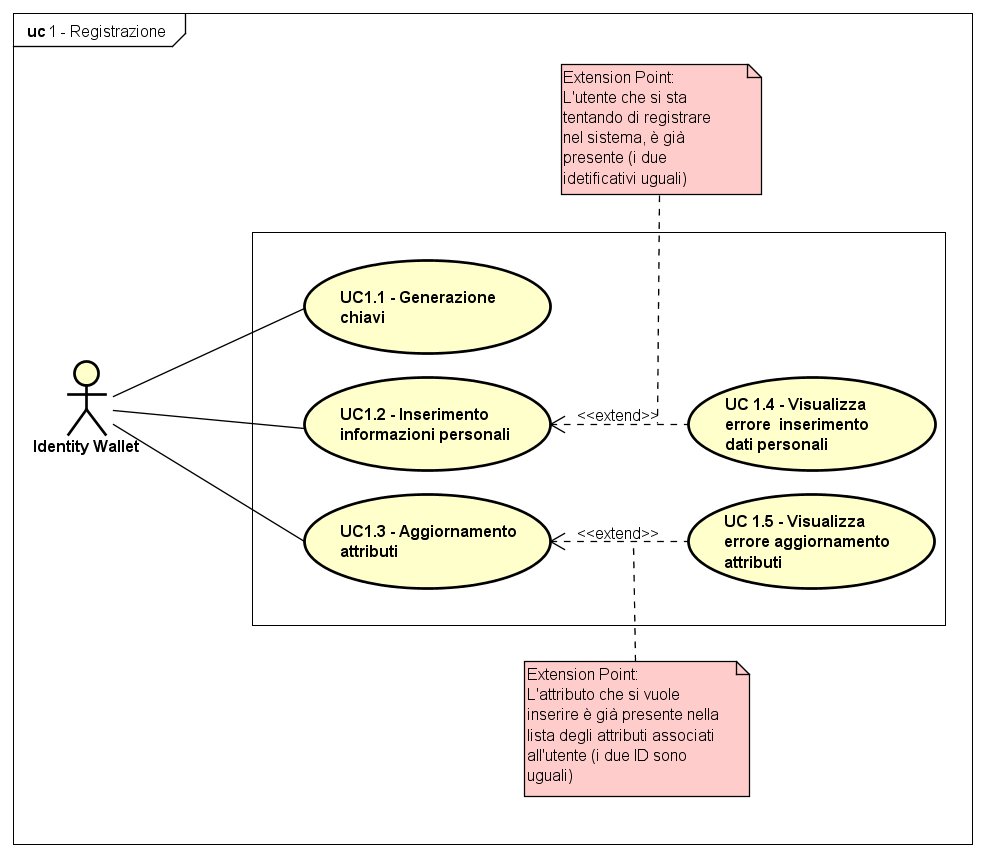
\includegraphics[scale=0.35]{immagini/usecase/UC1_Registrazione}
	\caption{Caso d'uso UC1: Registrazione}
\end{figure}
\begin{itemize}
	\item \textbf{Descrizione} - L'Identity Wallet genera la chiave pubblica, quella privata ed inserisce le informazioni personali dell'utente. In alternativa può aggiornare gli attributi esistenti aggiungendone di nuovi;
	\item \textbf{Attori Principali} - Identity Wallet;
	\item \textbf{Attori Secondari} - nessuno;
	\item \textbf{Pre-Condizioni} - L'Identity Wallet non possiede un'identità digitale per l'utente;
	\item \textbf{Post-Condizioni} - L'Identity Wallet ha creato un'identità per l'utente ed è in attesa che questa venga certificata;
	\item \textbf{Scenario Principale} - 
	\begin{enumerate}
		\item Generazione delle chiavi (UC 1.1);
		\item Inserimento delle informazioni personali (UC 1.2);
		\item Aggiornamento degli attributi già presenti nell'\gls{ITF} (UC 1.3);
	\end{enumerate}
	\item \textbf{Estensioni} -
	\begin{enumerate}
		\item All'Identity Wallet viene segnalato un errore di registrazione del nuovo utente (UC 1.4);
		\item All'Identity Wallet viene segnalato un errore sull'aggiornamento degli attributi (UC 1.5).
	\end{enumerate}
\end{itemize}
\newpage
\subsection{Caso d'uso UC1.1: Generazione Chiavi}
\begin{figure}[h]
	\centering
	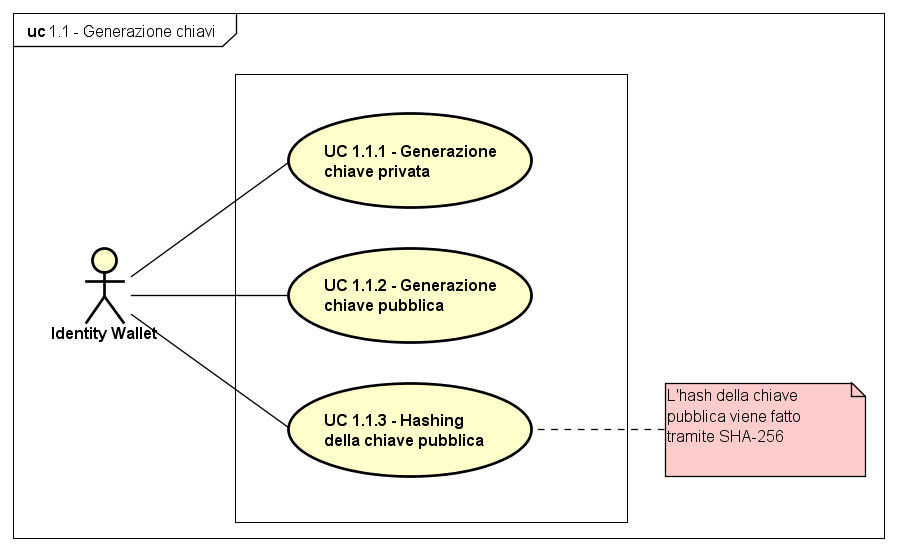
\includegraphics[scale=0.50]{immagini/usecase/UC11_GenerazioneChiavi}
	\caption{Caso d'uso UC1.1: Generazione chiavi}
\end{figure}
\begin{itemize}
	\item \textbf{Descrizione} - L'Identity Wallet genera la chiave privata e quella pubblica. Quest'ultima viene crittografata tramite \textit{hash} e rappresenta l'identità digitale dell'utente;
	\item \textbf{Attori Principali} - Identity Wallet;
	\item \textbf{Attori Secondari} - nessuno;
	\item \textbf{Pre-Condizioni} - L'Identity Wallet non possiede una coppia di chiavi pubblica-privata;
	\item \textbf{Post-Condizioni} - L'Identity Wallet è in possesso di una coppia di chiavi (pubblica e privata) e del \textit{hash} di quella pubblica;
	\item \textbf{Scenario Principale} -
	\begin{enumerate}
		\item Generazione della chiave privata (UC 1.1.1);
		\item Generazione della chiave pubblica (UC 1.1.2);
		\item Generazione del \textit{hash} della chiave pubblica (UC 1.1.3).
	\end{enumerate}
	\item \textbf{Estensioni} - non previste.
\end{itemize}
\newpage
\subsection{Caso d'uso UC1.2: Inserimento informazioni personali}
\begin{figure}[h]
	\centering
	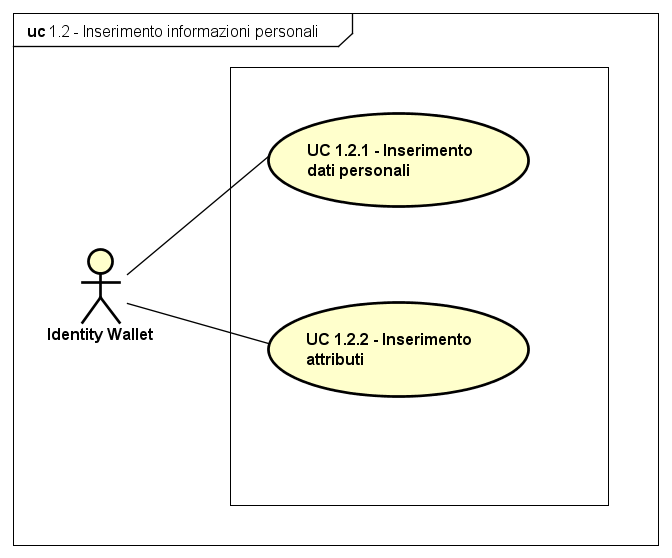
\includegraphics[scale=0.50]{immagini/usecase/UC12_InserimentoInformazioniPersonalii}
	\caption{Caso d'uso UC1.2: Inserimento informazioni personali}
\end{figure}
\begin{itemize}
	\item \textbf{Descrizione} - L'Identity Wallet crea l'identità digitale dell'utente come un insieme di dati personali e attributi a lui associati;
	\item \textbf{Attori Principali} - Identity Wallet;
	\item \textbf{Attori Secondari} - nessuno;
	\item \textbf{Pre-Condizioni} - L'Identity Wallet non possiede le informazioni personali dell'utente ed i suoi attributi;
	\item \textbf{Post-Condizioni} - L'Identity Wallet possiede tutte le informazioni personali dell'utente ed i suoi attributi;
	\item \textbf{Scenario Principale} -
	\begin{enumerate}
		\item Inserimento dei dati personali utente (UC 1.2.1);
		\item Inserimento dei degli attributi utente (UC 1.2.2);
	\end{enumerate}
	\item \textbf{Estensioni} - non previste.
\end{itemize}
\newpage
\subsection{Caso d'uso UC1.2.1: Inserimento dati personali utente}
\begin{figure}[h]
	\centering
	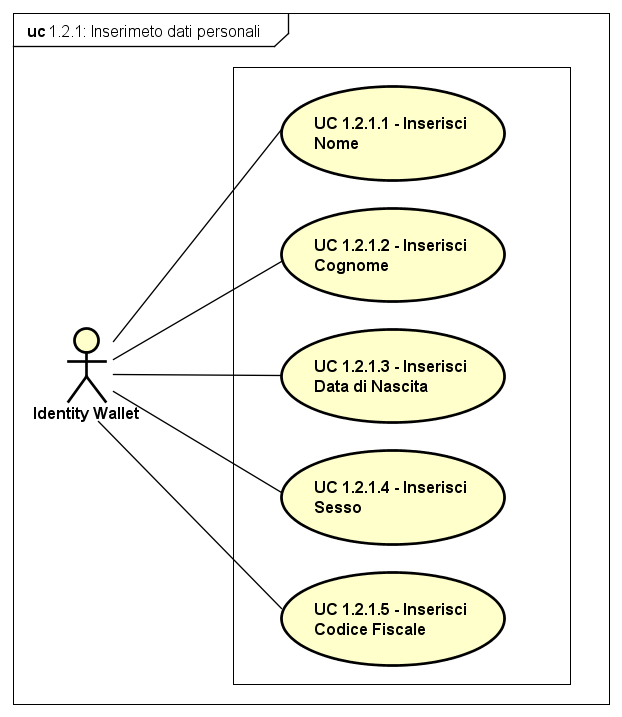
\includegraphics[scale=0.50]{immagini/usecase/UC121_InserimentoDatiPersonali}
	\caption{Caso d'uso UC1.2.1: Insierimento dati personali utente}
\end{figure}
\begin{itemize}
	\item \textbf{Descrizione} - L'Identity Wallet compila i campi dedicati alle informazioni personali dell'identità utente che vuole registrare all'ITF;
	\item \textbf{Attori Principali} - Identity Wallet;
	\item \textbf{Attori Secondari} - nessuno;
	\item \textbf{Pre-Condizioni} - L'Identity Wallet non ha inserito le informazioni personali dell'identità utente che vuole registrare nell'\gls{ITF};
	\item \textbf{Post-Condizioni} - L'Identity Wallet ha inserito tutte le informazioni personali dell'identità utente che vuole registrare nell'\gls{ITF};
	\item \textbf{Scenario Principale} -
	\begin{enumerate}
		\item Inserimento del nome dell'utente (UC 1.2.1.1);
		\item Inserimento del cognome dell'utente (UC 1.2.1.2);
		\item Inserimento della data di nascita (UC 1.2.1.3);
		\item Inserimento del sesso dell'utente (UC 1.2.1.4);
		\item Inserimento del codice fiscale (UC 1.2.1.5).
	\end{enumerate}
	\item \textbf{Estensioni} - non previste.
\end{itemize}
\newpage
\subsection{Caso d'uso UC1.2.2: Inserimento attributi}
\begin{figure}[h]
	\centering
	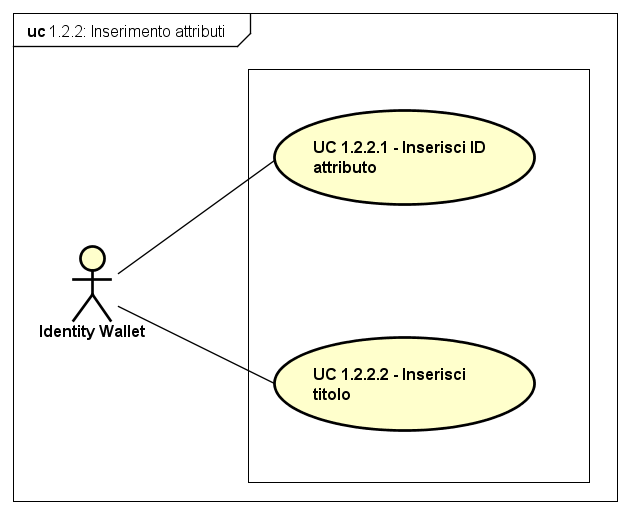
\includegraphics[scale=0.50]{immagini/usecase/UC122_InserimentoAttributi}
	\caption{Caso d'uso UC1.2.2: Inserimento attributi}
\end{figure}
\begin{itemize}
	\item \textbf{Descrizione} -L'Identity Wallet compila i campi dedicati agli attributi/certificazioni per creare l'identità digitale dell'utente;
	\item \textbf{Attori Principali} - Identity Wallet;
	\item \textbf{Attori Secondari} - nessuno;
	\item \textbf{Pre-Condizioni} - L'Identity Wallet non possiede le informazioni inerenti agli attributi/certificazioni dell'utente che sta registrando nell'\gls{ITF};
	\item \textbf{Post-Condizioni} - L'Identity Wallet possiede tutte le informazioni inerenti agli attributi/certificazioni dell'utente che sta registrando nell'\gls{ITF};
	\item \textbf{Scenario Principale} -
	\begin{enumerate}
		\item Inserimento dell'ID che individua l'attributo (UC 1.2.2.1);
		\item Inserimento del titolo che descrive l'attributo (UC 1.2.2.2).
	\end{enumerate}
	\item \textbf{Estensioni} - non previste.
\end{itemize}
\newpage
\subsection{Caso d'uso UC1.3: Aggiornamento attributi}
\begin{figure}[h]
	\centering
	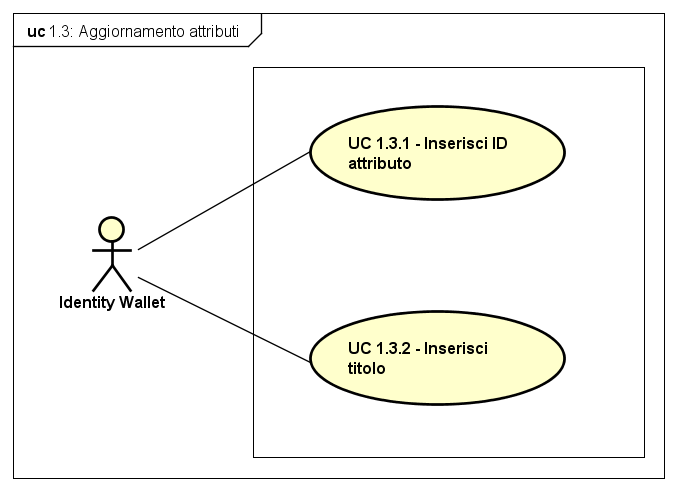
\includegraphics[scale=0.50]{immagini/usecase/UC13_AggiornamentoAttributi}
	\caption{Caso d'uso UC1.3: Aggiornamento attributi}
\end{figure}
\begin{itemize}
	\item \textbf{Descrizione} - L'Identity Wallet aggiorna gli attributi/certificazioni dell'utente, aggiungendone di nuove alla lista di quelle già presente nell'\gls{ITF};
	\item \textbf{Attori Principali} - Identity Wallet;
	\item \textbf{Attori Secondari} - nessuno;
	\item \textbf{Pre-Condizioni} - L'Identity Wallet vuole aggiornare la lista di attributi/certificazioni associati all'utente;
	\item \textbf{Post-Condizioni} - L'Identity Wallet ha aggiornato la lista di attributi/certificazioni associati all'utente;
	\item \textbf{Scenario Principale} -
	\begin{enumerate}
		\item Inserimento dell'ID corrispondente all'attributo (UC 1.3.1);
		\item Inserimento del titolo descrittivo dell'attributo (UC 1.3.2).
	\end{enumerate}
	\item \textbf{Estensioni} - non previste.
\end{itemize}
\subsection{Caso d'uso UC1.4: Visualizza errore registrazione utente}
\begin{itemize}
	\item \textbf{Descrizione} - All'Identity Wallet viene segnalata, tramite un opportuno errore, l'impossibilità di creare e registrare una nuova identità digitale per l'utente. Questo avviene quando si tenta di registrare un'identità che è già presente nel sistema;
	\item \textbf{Attori Principali} - Identity Wallet;
	\item \textbf{Attori Secondari} - nessuno;
	\item \textbf{Pre-Condizioni} - L'Identity Wallet vuole registrare una nuova identità digitale per l'utente;
	\item \textbf{Post-Condizioni} - L'Identity Wallet non è riuscito a registrare la nuova identità digitale nell'\gls{ITF};
	\item \textbf{Scenario Principale} -
	\begin{enumerate}
		\item All'Identity Wallet viene segnalata, tramite un errore, l'impossibilità di registrare il nuovo utente al sistema (UC 1.4);
	\end{enumerate}
	\item \textbf{Estensioni} - non previste.
\end{itemize}
\subsection{Caso d'uso UC1.5: Visualizza errore aggiornamento attributo}
\begin{itemize}
	\item \textbf{Descrizione} - All'Identity Wallet viene segnalata, tramite un opportuno errore, l'impossibilità di aggiornare la lista di attributi/certificazioni dell'utente. Questo avviene quando si tenta di aggiornare un attributo/certificazione che non è presente nell'\gls{ITF};
	\item \textbf{Attori Principali} - Identity Wallet;
	\item \textbf{Attori Secondari} - nessuno;
	\item \textbf{Pre-Condizioni} - L'Identity Wallet vuole aggiornare la lista degli attributi e certificazioni associati all'utente;
	\item \textbf{Post-Condizioni} - La lista non è stata aggiornata;
	\item \textbf{Scenario Principale} -
	\begin{enumerate}
		\item All'Identity Wallet viene segnalata, tramite un errore, l'impossibilità di aggiornare gli attributi (UC 1.5);
	\end{enumerate}
	\item \textbf{Estensioni} - non previste.
\end{itemize}
\newpage
\subsection{Caso d'uso UC2: Certificazione}
\begin{figure}[h]
	\centering
	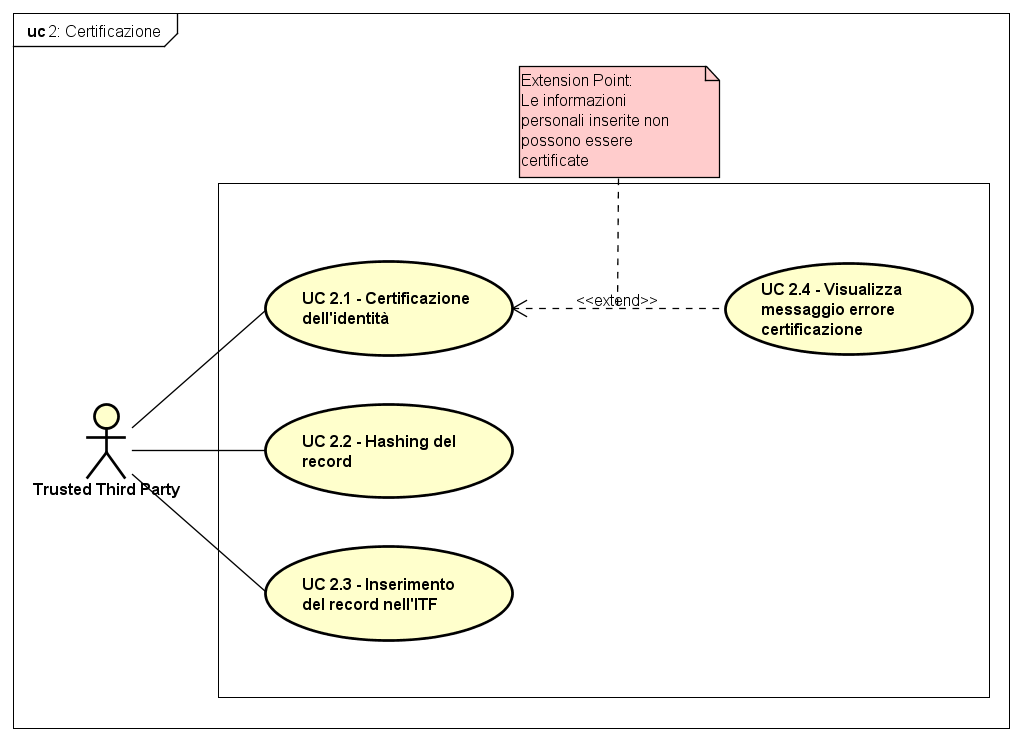
\includegraphics[scale=0.50]{immagini/usecase/UC2_Certificazione}
	\caption{Caso d'uso UC2: Certificazione}
\end{figure}
\begin{itemize}
	\item \textbf{Descrizione} - L'attore vuole certificare tutte le informazioni riguardanti l'identità digitale dell'utente e, una volta certificate, inserirle nell'\gls{ITF}.\\
	La certificazione avviene grazie alla firma, delle informazioni personali e degli attributi, tramite la chiave privata dell'attore. Una volta firmate, le informazioni vengono inserite in un record, fatto l'\textit{hash} del record e quindi inserito nell'\gls{ITF};	
	\item \textbf{Attori Principali} - Trusted Third Party;
	\item \textbf{Attori Secondari} - nessuno;
	\item \textbf{Pre-Condizioni} - L'attore vuole certificare l'identità e gli attributi di un particolare utente;
	\item \textbf{Post-Condizioni} - La Trusted Third Party ha certificato correttamente l'identità e gli attributi dell'utente e ha inserito il record nell'\gls{ITF};
	\item \textbf{Scenario Principale} -
	\begin{enumerate}
		\item L'attore certifica le informazioni dell'utente (UC 2.1);
		\item L'attore esegue l'\textit{hash} del record contenente tutte le informazioni appena certificate (UC 2.2);
		\item L'attore, una volta fatto l'\textit{hash} del record, lo inserisce nell'\gls{ITF} (UC 2.3).
	\end{enumerate}
	\item \textbf{Estensioni} -
	\begin{enumerate}
		\item Visualizza messaggio d'errore nella certificazione delle informazioni personali (UC 2.4).
	\end{enumerate}
\end{itemize}
\subsection{Caso d'uso UC2.1: Certificazione dell'identità}
\begin{figure}[h]
	\centering
	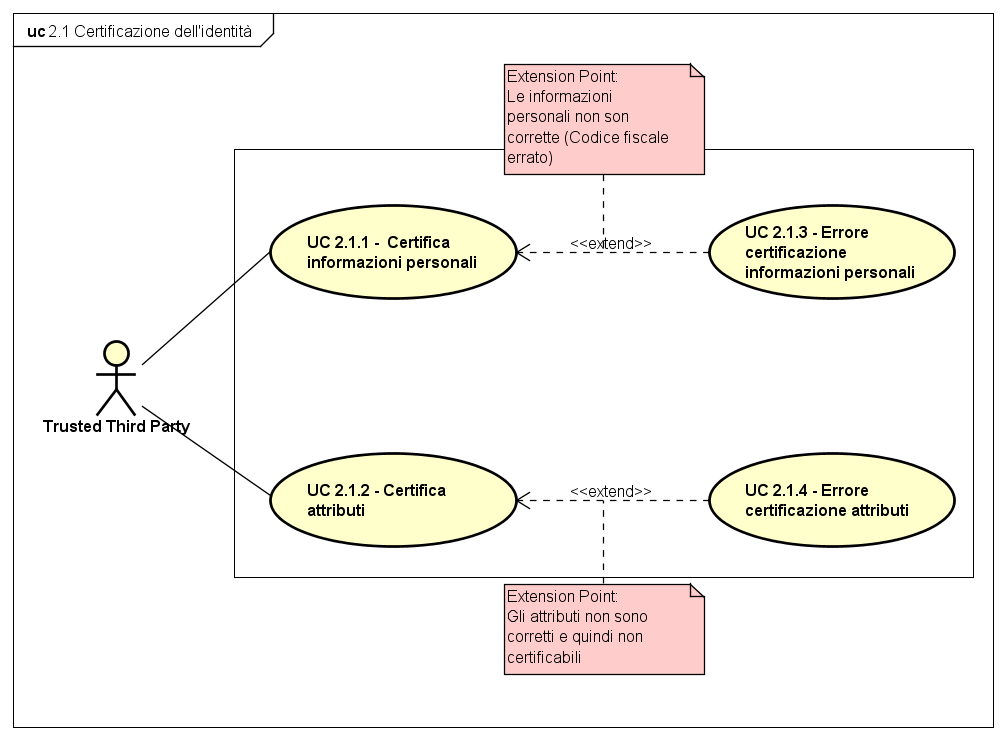
\includegraphics[scale=0.50]{immagini/usecase/UC21_CertificazioneIdentita}
	\caption{Caso d'uso UC2.1: Certificazione dell'identità}
\end{figure}
\begin{itemize}
	\item \textbf{Descrizione} - La Trusted Third Party, prima di inserire il record nell'ITF, deve certificare tutte le informazioni personali associate all'utente (dati e attributi/certificazioni).\\
	Questo viene fatto grazie alla firma dei dati e degli attributi tramite chiave privata della Trusted Third Party;
	\item \textbf{Attori Principali} - Trusted Third Party;
	\item \textbf{Attori Secondari} - nessuno;
	\item \textbf{Pre-Condizioni} - L'attore vuole certificare tutte le informazioni personali dell'utente;
	\item \textbf{Post-Condizioni} - L'attore ha certificato tutte le informazioni personali dell'utente;
	\item \textbf{Scenario Principale} -
	\begin{enumerate}
		\item Certificazione delle informazioni personali tramite chiave privata (UC 2.1.1);
		\item Certificazione degli attributi/certificazioni tramite chiave privata (UC 2.1.2).
	\end{enumerate}
	\item \textbf{Estensioni} -
	\begin{enumerate}
		\item Visualizza errore nella certificazione delle informazioni personali (UC 2.1.3);
		\item Visualizza errore nella certificazione degli attributi (UC 2.1.4).
	\end{enumerate}
\end{itemize}
\subsection{Caso d'uso UC 2.4: Visualizza errore certificazione dell'identità}
\begin{itemize}
	\item \textbf{Descrizione} - Alla Trusted Third Party viene segnalata l'impossibilità di certificare uno o più informazioni personali dell'utente (dati personali, attributo o certificazioni).\\
	Questo avviene quando la Trusted Third Party non riesce a trovare corrispondenza tra gli attributi e i dati indicati con l'identità dell'utente;
	\item \textbf{Attori Principali} - Trusted Third Party;
	\item \textbf{Attori Secondari} - nessuno;
	\item \textbf{Pre-Condizioni} - L'attore vuole certificare tutte le informazioni personali dell'utente (dati personali e attributi);
	\item \textbf{Post-Condizioni} - L'attore non è riuscito a certificare gli attributi e/o i dati personali dell'utente;
	\item \textbf{Scenario Principale} -
	\begin{enumerate}
		\item L'attore viene segnalato dell'impossibilità di certificare le informazioni personali dell'utente tramite un apposito errore (UC 2.4).
	\end{enumerate}
	\item \textbf{Estensioni} - non previste.
\end{itemize}
\subsection{Caso d'uso UC 2.1.3: Visualizza errore certificazione informazioni personali}
\begin{itemize}
	\item \textbf{Descrizione} - Alla Trusted Third Party viene segnalata l'impossibilità di certificare le informazioni personali dell'utente;
	\item \textbf{Attori Principali} - Trusted Third Party
	\item \textbf{Attori Secondari} - nessuno;
	\item \textbf{Pre-Condizioni} - L'attore vuole certificare le informazioni personali dell'utente;
	\item \textbf{Post-Condizioni} - L'attore non è riuscito a certificare le informazioni personali dell'utente;
	\item \textbf{Scenario Principale} -
	\begin{enumerate}
		\item L'attore viene segnalato dell'impossibilità di certificare le informazioni personali, tramite un apposito errore (UC 2.1.3).
	\end{enumerate}
	\item \textbf{Estensioni} - non previste.
\end{itemize}
\subsection{Caso d'uso UC 2.1.4: Visualizza errore certificazione attributi}
\begin{itemize}
	\item \textbf{Descrizione} - Alla Trusted Third Party viene segnalata l'impossibilità di certificare gli attributi dell'utente;
	\item \textbf{Attori Principali} - Trusted Third Party;
	\item \textbf{Attori Secondari} - nessuno;
	\item \textbf{Pre-Condizioni} - L'attore vuole certificare gli attributi dell'utente;
	\item \textbf{Post-Condizioni} - L'attore non è riuscito a certificare gli attributi dell'utente;
	\item \textbf{Scenario Principale} - 
	\begin{enumerate}
		\item L'attore viene segnalato dell'impossibilità di certificare gli attributi, tramite un apposito errore (UC 2.1.4).
	\end{enumerate}
	\item \textbf{Estensioni} - non previste.
\end{itemize}
\subsection{Caso d'uso UC3: Verifica delle informazioni utente}
\begin{figure}[h]
	\centering
	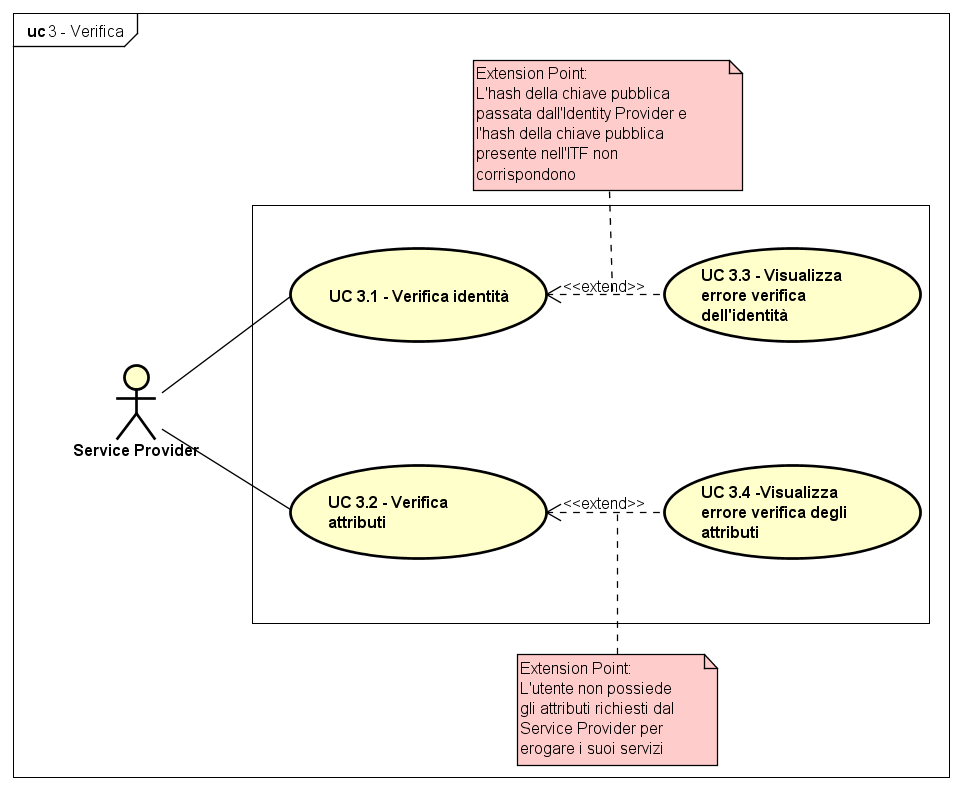
\includegraphics[scale=0.50]{immagini/usecase/UC3_Verifica}
	\caption{Caso d'uso UC3: Verifica}
\end{figure}
\begin{itemize}
	\item \textbf{Descrizione} - Il Service Provider, prima di poter erogare i suoi servizi, deve accertarsi che l'utente sia in possesso delle credenziali e degli attributi necessari. Questo avviene tramite la verifica dell'identità e la verifica degli attributi presenti nell'\gls{ITF};
	\item \textbf{Attori Principali} -Service Provider;
	\item \textbf{Attori Secondari} - nessuno;
	\item \textbf{Pre-Condizioni} - Il Service Provider non ha verificato l'identità e gli attributi dell'utente;
	\item \textbf{Post-Condizioni} - Il Service Provider ha verificato l'identità dell'utente e può erogare i suoi servizi;
	\item \textbf{Scenario Principale} -
	\begin{enumerate}
		\item Verifica dell'identità dell'utente (UC 3.1);
		\item Verifica degli attributi dell'utente (UC 3.2).
	\end{enumerate}
	\item \textbf{Estensioni} -
	\begin{enumerate}
		\item Visualizza errore nella verifica dell'identità (UC 3.3);
		\item Visualizza errore nella verifica degli attributi (UC 3.4).
	\end{enumerate}
\end{itemize}
\subsection{Caso d'uso UC3.1: Verifica identità}
\begin{figure}[h]
	\centering
	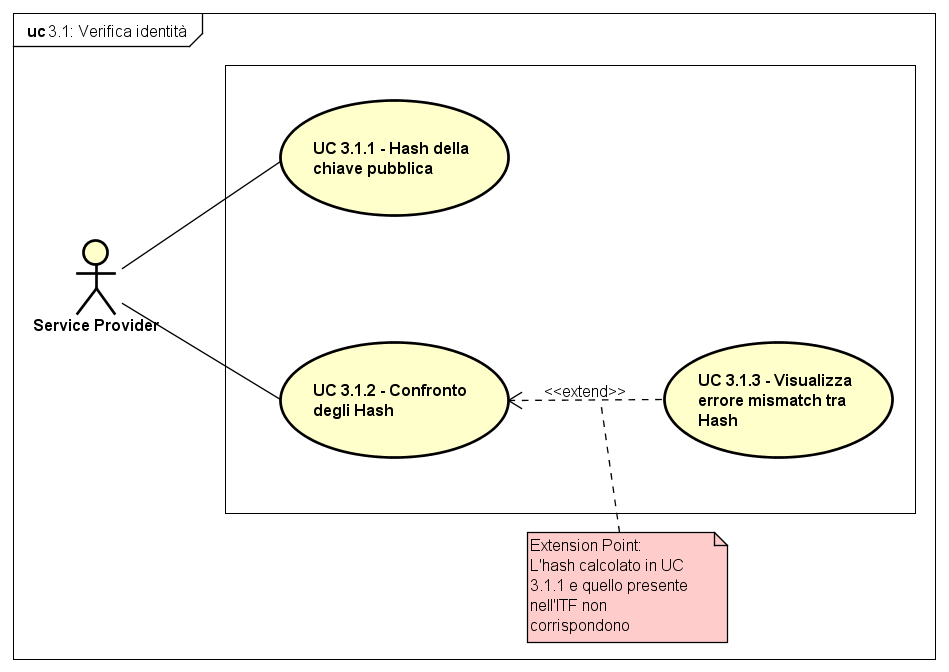
\includegraphics[scale=0.50]{immagini/usecase/UC31_VerificaIdentita}
	\caption{Caso d'uso UC3.1: Verifica dell'identità}
\end{figure}
\begin{itemize}
	\item \textbf{Descrizione} -  Il Service Provider, prima di permettere all'utente di usufruire dei suoi servizi, deve accertarsi che l'identità dell'utente sia corretta rispetto a quella presente nell'\gls{ITF};
	\item \textbf{Attori Principali} - Service Provider;
	\item \textbf{Attori Secondari} - nessuno;
	\item \textbf{Pre-Condizioni} - L'attore non sa se può erogare i servizi all'utente;
	\item \textbf{Post-Condizioni} - Il Service Provider ha verificato l'identità dell'utente e può erogare i suoi servizi;
	\item \textbf{Scenario Principale} -
	\begin{enumerate}
		\item \textit{Hash} della chiave pubblica passata dall'Idenitity Wallet (UC 3.1.1);
		\item Confronto del \textit{hash} calcolato in UC 3.1.1 con quello presente nell'\gls{ITF} (UC 3.1.2).
	\end{enumerate}
	\item \textbf{Estensioni} -
	\begin{enumerate}
		\item Visualizza errore mismatch degli hash (UC 3.1.3).
	\end{enumerate}
\end{itemize}
\subsection{Caso d'uso UC3.3: Visualizza errore verifica identità}
\begin{itemize}
	\item \textbf{Descrizione} - Il Service Provider, prima di poter erogare i suoi servizi, deve verificare che l'identità utente sia certificata e quindi presente nell'\gls{ITF}.\\
	Se questo non avviene, allora il Service Provider non deve erogare nessun servizio all'utente che li richiede.\\
	Specificato meglio in caso d'uso UC3.1.3;
	\item \textbf{Attori Principali} - Service Provider;
	\item \textbf{Attori Secondari} - nessuno;
	\item \textbf{Pre-Condizioni} - Il Service Provider è in attesa della verifica delle informazioni utente per erogare i suoi servizi;
	\item \textbf{Post-Condizioni} - Il Service Provider non è riuscito a verificare l'identità utente;
	\item \textbf{Scenario Principale} -
	\begin{enumerate}
		\item Viene visualizzato un errore di verifica dell'identità (UC 3.3).
	\end{enumerate}
	\item \textbf{Estensioni} - non previste.
\end{itemize}
\subsection{Caso d'uso UC3.1.3: Visualizza errore mismatch hash}
\begin{itemize}
	\item \textbf{Descrizione} - Il Service Provider, prima di poter erogare i suoi servizi, deve verificare che l'identità dell'utente sia corretta. Questo viene fatto tramite confronto degli \textit{hash}.\\
	Gli \textit{hash} da confrontare sono: quello presente nell'\gls{ITF} (certificato) e quello calcolato a partire dalla chiave pubblica che il Service Provider ha ottenuto dall'Identity Wallet.\\
	Se i due \textit{hash} non sono uguali significa che quello ottenuto dall'Identity Wallet non è corretto. Questo viene segnalato tramite un opportuno messaggio d'errore;
	\item \textbf{Attori Principali} - Service Provider
	\item \textbf{Attori Secondari} - nessuno;
	\item \textbf{Pre-Condizioni} - L'attore è in attesa della verifica delle informazioni utente per erogare i suoi servizi;
	\item \textbf{Post-Condizioni} - L'attore, non essendo riuscito a verificare l'identità dell'utente, non può erogare i suoi servizi;
	\item \textbf{Scenario Principale} - 
	\begin{enumerate}
		\item Visualizza un opportuno errore di mismatch tra gli \textit{hash} delle chiavi pubbliche (UC 3.1.3).
	\end{enumerate}
	\item \textbf{Estensioni} - non previste.
\end{itemize}
\subsection{Caso d'uso UC3.4: Visualizza errore verifica degli attributi}
\begin{itemize}
	\item \textbf{Descrizione} - Il Service Provider deve, per poter erogare i suoi servizi, verificare l'identità e gli attributi dell'utente.\\
	L'identità viene spiegata in UC3.1, UC3.3 e in UC3.1.3.\\
	In questo caso, si ha come precondizione che l'identità sia stata verificata.
	Per poter erogare i servizi, il Service Provider deve assicurarsi che l'utente sia in possesso degli attributi necessari che ne permettono l'autorizzazione all'utilizzo.\\
	Questo viene fatto andando a confrontare una lista di attributi, richiesti dal Service Provider, con la lista di attributi associati all'utente presente nell'\gls{ITF}.\\
	Essendo presente nell'\gls{ITF} vuol dire che la lista è composta solo da attributi certificati da una terza parte fidata.\\
	Se gli attributi richiesti dal Service Provider non son presenti, del tutto o in parte, nella lista degli attributi certificati dell'utente, il Service Provider non eroga nessun servizio;
	\item \textbf{Attori Principali} - Service Provider;
	\item \textbf{Attori Secondari} - nessuno;
	\item \textbf{Pre-Condizioni} - Il Service Provider ha verificato correttamente l'identità dell'utente ma non sa se è in possesso degli attributi necessari per poter accedere ai suoi servizi;
	\item \textbf{Post-Condizioni} - Il Service Provider non è riuscito a verificare gli attributi dell'utente quindi non può erogare i suoi servizi in quanto non è autorizzato ad accedervi;
	\item \textbf{Scenario Principale} -
	\begin{enumerate}
		\item Visualizza un opportuno messaggio d'errore per la verifica degli attributi (UC 3.4).
	\end{enumerate}
	\item \textbf{Estensioni} - non previste.
\end{itemize}
\newpage
\subsection{Caso d'uso UC4: Aggiornamento degli attributi}
\begin{figure}[h]
	\centering
	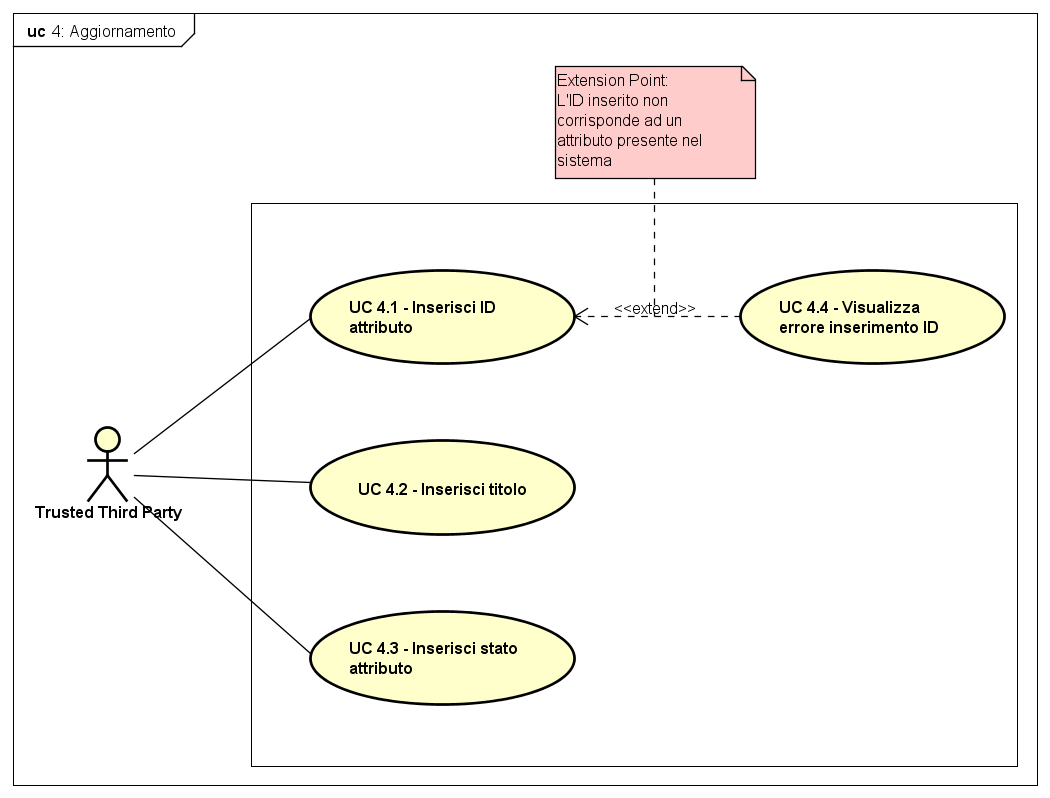
\includegraphics[scale=0.50]{immagini/usecase/UC4_Aggiornamento}
	\caption{Caso d'uso UC4: Aggiornamento}
\end{figure}
\begin{itemize}
	\item \textbf{Descrizione} -La Trusted Third Party, su richiesta dell'utente o non, deve aggiornare lo stato di un attributo o asserzione dell'utente stesso.
	Questo viene fatto creando un nuovo blocco che rappresenta l'attributo della quale si vuole fare l'aggiornamento. In questo nuovo blocco vengono inseriti: l'ID del vecchio blocco che si vuole aggiornare, la nuova descrizione dell'attributo e lo stato dell'attributo (ovvero se l'attributo è valido, se è all'ultima versione disponibile ecc..).\\
	Una volta creato il blocco verrà aggiunto un timestamp ed il nuovo blocco aggiunto alla catena.\\
	Quando un Service Provider vuole recuperare le informazioni riguardanti l'utente dovrà prendere il blocco con timestamp più recente. Questo tipo di aggiornamento fa sì che i nuovi blocchi "oscurino" quelli vecchi.\\
	I vecchi blocchi son comunque recuperabili grazie al riferimento che i nuovi blocchi hanno verso di loro. Questo permette la realizzazione di uno storico delle certificazioni prese da un utente e dello stato di avanzamento del \textit{Trust} che un utente ha nei confronti della rete;
	\item \textbf{Attori Principali} - Trusted Third Party;
	\item \textbf{Attori Secondari} - nessuno;
	\item \textbf{Pre-Condizioni} - La Trusted Third Party vuole o deve, su richiesta dell'utente, aggiornare lo stato di un attributo che ha già certificato;
	\item \textbf{Post-Condizioni} - La Trusted Third Party è riuscita ad aggiornare lo stato di un attributo già certificato ;
	\item \textbf{Scenario Principale} -
	\begin{enumerate}
		\item Inserimento ID dell'attributo da aggiornare (UC 4.1);
		\item Inserimento del nuovo titolo descrittivo (UC 4.2);
		\item Inserimento dello stato del nuovo attributo (UC 4.3).
	\end{enumerate}
	\item \textbf{Estensioni} -
	\begin{enumerate}
		\item VIsualizza errore nell'inserimento ID (UC 4.4).
	\end{enumerate}
\end{itemize}
\subsection{Caso d'uso UC4.4: Visualizza errore inserimento ID}
\begin{itemize}
	\item \textbf{Descrizione} - La Trusted Third Party deve, su richiesta dell'utente o per sua volontà, aggiornare lo stato di una certificazione.\\
	Questo avviene inserendo l'ID della certificazione che si vuole aggiornare ed aggiornando il titolo e lo stato. In automatico verrà posto un timestamp più recente che andrà ad "oscurare" le certificazioni meno recenti.\\
	L'errore viene scatenato quando si tenta di aggiornare un attributo che non esiste o non è presente nel sistema (ID errato);
	\item \textbf{Attori Principali} - Trusted Third Party;
	\item \textbf{Attori Secondari} - nessuno;
	\item \textbf{Pre-Condizioni} - La Trusted Third Party vuole o deve, su richiesta dell'utente, aggiornare lo stato di un attributo che ha già certificato;
	\item \textbf{Post-Condizioni} - La Trusted Third Party non è riuscita ad aggiornare lo stato dell'attributo richiesto;
	\item \textbf{Scenario Principale} -
	\begin{enumerate}
		\item Visualizza errore inserimento ID (UC 4.4).
	\end{enumerate}
	\item \textbf{Estensioni} - non previste.
\end{itemize}
\newpage
\subsection{Caso d'uso UC5: Revoca della certificazione}
\begin{figure}[h]
	\centering
	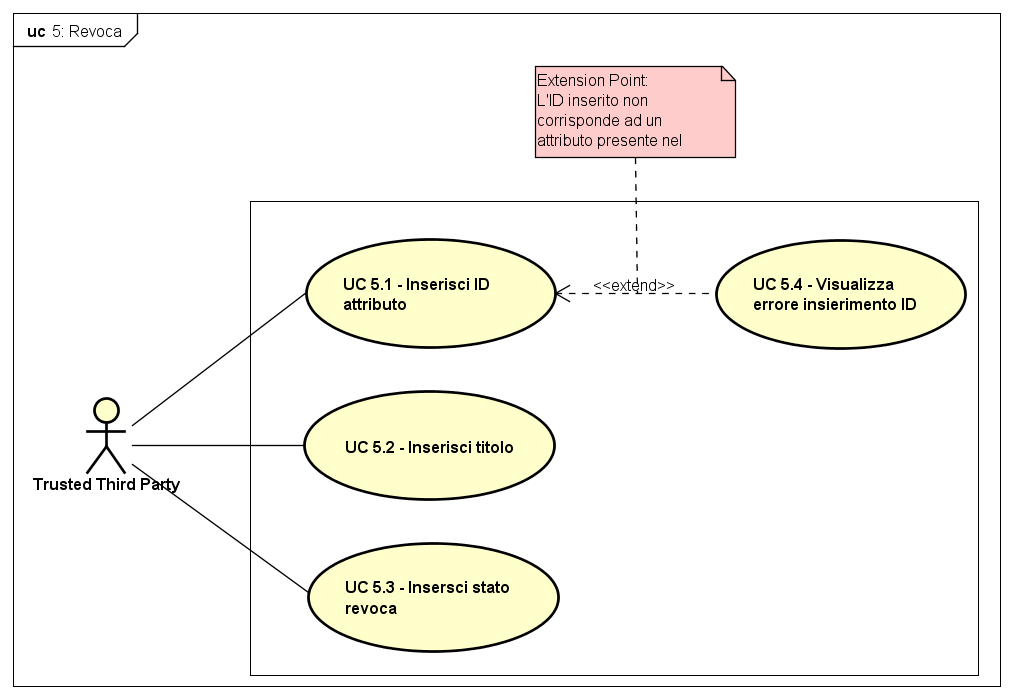
\includegraphics[scale=0.50]{immagini/usecase/UC5_Revoca}
	\caption{Caso d'uso UC5: Revoca}
\end{figure}
\begin{itemize}
	\item \textbf{Descrizione} - La Trusted Third Party può decidere di revocare una certificazione o un attributo che prima aveva certificato. Questo può avvenire per scadenza della certificazione o per ritiro da parte di enti terzi.\\
	Le dinamiche sono le stesse dell'aggiornamento (caso d'uso UC4) con la differenza che, lo stato viene utilizzato per indicare se un attributo è ancora valido o meno.\\
	Anche in questo caso il nuovo blocco inserito andrà ad "oscurare" tutti i blocchi con un timestamp più vecchio e sarà il Service Provider a dover recuperare i blocchi con timestamp più recente.\\
	Come nell'aggiornamento del UC4, anche qui è possibile ottenere uno storico delle certificazioni così da poter visualizzare il loro stato di avanzamento fino alla loro revoca;
	\item \textbf{Attori Principali} - Trusted Third Party;
	\item \textbf{Attori Secondari} - nessuno;
	\item \textbf{Pre-Condizioni} - La Trusted Third Party deve revocare una particolare certificazione di un utente specifico;
	\item \textbf{Post-Condizioni} - La Trusted Third Party è riuscita a revocare la certificazione richiesta;
	\item \textbf{Scenario Principale} -
	\begin{enumerate}
		\item Inserimento dell'ID dell'attributo da rimuovere (UC 5.1);
		\item Inserimento del titolo dell'attributo da rimuovere (UC 5.2);
		\item Inserimento dello stato della revoca (UC 5.3).
	\end{enumerate}
	\item \textbf{Estensioni} -
	\begin{enumerate}
		\item Visualizza errore nell'inserimento dell'ID (UC 5.4).
	\end{enumerate}
\end{itemize}
\subsection{Caso d'uso UC5.4: Visualizza messaggio d'errore inserimento ID}
\begin{itemize}
	\item \textbf{Descrizione} - La Trusted Third Party deve revocare una certificazione.\\
	Questo avviene inserendo l'ID della certificazione che si vuole revocare ed inserendo un codice prefissato nello stato. In automatico verrà posto un timestamp più recente che andrà ad "oscurare" le certificazioni meno recenti.\\
	L'errore viene scatenato quando si tenta di revocare un attributo che non esiste o non è presente nel sistema (ID errato);	
	\item \textbf{Attori Principali} - Trusted Third Party;
	\item \textbf{Attori Secondari} - nessuno;
	\item \textbf{Pre-Condizioni} - La Trusted Third Party deve revocare una certificazione sepcifica dell'utente;
	\item \textbf{Post-Condizioni} - La Trusted Third Party non è riuscita a revocare la certificazione dell'utente;
	\item \textbf{Scenario Principale} -
	\begin{enumerate}
		\item Visualizza errore inserimento ID (UC 5.4).
	\end{enumerate}
	\item \textbf{Estensioni} - non previste.
\end{itemize}
\section{Requisiti}
In questa sezione verranno elencati e descritti tutti i requisiti rilevati durante la fase di analisi dei requisiti. Questi saranno inseriti all'interno di una tabella contenente:
\begin{itemize}
	\item ID del requisito;
	\item Breve descrizione del requisito;
	\item Fonti dov'è possibile trovare o ricondursi al requisito stesso.
\end{itemize}
Prima di questo, verrà spiegata la nomenclatura adottata al fine di catalogare, ordinare e tracciare tutti i requisiti.
\subsection{Classificazione dei requisiti}
Ogni requisito viene classificato secondo la seguente convenzione:\\
\centerline{R[Tipologia][Importanza]][Padre].[Livello]}\\
\begin{itemize}
	\item \textbf{Tipologia} - Indica la tipologia del requisito indicata con una lettera tra:
	\begin{itemize}
		\item \textbf{F}: \textit{Funzionale}, ovvero le funzionalità che il sistema offre;
		\item \textbf{P}: \textit{Prestazionale}, ovvero i vincoli sulle prestazioni che il sistema deve soddisfare;
		\item \textbf{Q}: \textit{Qualità}, ovvero specifica i vincoli di qualità che il sistema deve soddisfare;
		\item \textbf{V}: \textit{Vincolo}, ovvero rappresenta tutti i vincoli non funzionali che dipendono da fattori esterni, legali e di dominio.
	\end{itemize}
	\item \textbf{Importanza} - Indica l'importanza del requisito o la sua utilità strategica. Viene rappresentata da una lettera maiuscola tra:
	\begin{itemize}
		\item \textbf{O}: Rappresenta un requisito \textit{Obbligatorio} che deve essere soddisfatto per garantire le funzionalità base del sistema;
		\item \textbf{D}: Rappresenta un requisito \textit{Desiderabile} il cui non soddisfacimento non pregiudica le funzionalità del sistema ma, la sua realizzazione, da un valore aggiunto rendendo il tutto più completo;
		\item \textbf{F}: Rappresenta un requisito \textit{Facoltativo} che, se soddisfatto, renderebbe il sistema ancora più completo a discapito di risorse e aumento dei potenziali costi.
	\end{itemize}
	\item \textbf{Padre} - Numero che rappresenta univocamente un requisito;
	\item \textbf{Livello} - Per ogni "padre", il livello indica il numero del sotto requisito del caso preso in esame.
\end{itemize}
\subsection{Requisiti Funzionali}
\begin{longtable}{|r l|p{10cm}|p{2cm}|}
	\hline
	\multicolumn{2}{|c|}{\textbf{ID Requisito}} & \textbf{Descrizione} & \textbf{Fonti}\tabularnewline
	\hline
	&\textbf{RFO1.0}&Il sistema richiede che l'identità digitale venga generata&UC1 \\\hline
	&\textbf{RFO2.0}&Il sistema richiede la generazione delle chiavi pubbliche&UC1, UC1.1 \\\hline
	&\textbf{RFO3.0}&Il sistema richiede la generazione delle chiavi private&UC1, UC1.1 \\\hline
	&\textbf{RFO4.0}&Il sistema richiede l'inserimento delle informazioni personali dell'utente&UC1, UC1.2, UC1.2.1, UC1.2.2 \\\hline
	&\textbf{RFO4.1}&Il sistema richiede l'inserimento dei dati personali utente&UC1, UC1.2, UC1.2.1 \\\hline
	&\textbf{RFO4.1.1}&Il sistema richiede l'inserimento di un identificativo&UC1.2, UC1.2.1 \\\hline
	&\textbf{RFO4.1.2}&Il sistema richiede l'inserimento della data di nascita&UC1.2, UC1.2.1 \\\hline
	&\textbf{RFO4.1.3}&Il sistema richiede l'inserimento del sesso ("M" per maschio o "F" per femmina)&UC1.2, UC1.2.1\\\hline
	&\textbf{RFO4.1.4}&Il sistema richiede l'inserimento del nome da associare all'identità digitale&UC1.2.1, UC1.2.1.1\\\hline
	&\textbf{RFO4.1.5}&Il sistema richiede l'inserimento del cognome da associare all'identità digitale&UC1.2.1, UC1.2.1.2\\\hline
	&\textbf{RFO4.2}&Il sistema richiede l'inserimento degli attributi associati all'utente&UC1, UC1.2, UC1.2.2 \\\hline
	&\textbf{RFO4.2.1}&Il sistema richiede l'inserimento di un identificativo per l'attributo&UC1.2.2, UC1.2.2.1 \\\hline
	&\textbf{RFO4.2.1.1}& L'identificativo associato all'attributo deve essere univoco&UC1.2.2, UC1.2.2.1 \\\hline
	&\textbf{RFO4.2.2}&Ad ogni attributo va associato un titolo che lo descrive&UC1.2.2, UC1.2.2.2 \\\hline
	&\textbf{RFO5.0}&Il sistema genera un messaggio d'errore nel caso in cui ci siano problemi durante la registrazione&UC1, UC1.4 \\\hline
	&\textbf{RFO6.0}&Il sistema permette l'aggiornamento degli attributi associati ad un utente&UC1, UC1.3 \\\hline
	&\textbf{RFO6.1}&Il sistema richiede l'inserimento di un'identificativo per l'attributo&UC1.3, UC1.3.1 \\\hline
	&\textbf{RFO6.1.1}&Il sistema richiede l'inserimento di un ID univoco associato ad un attributo&UC1.3, UC1.3.1 \\\hline
	&\textbf{RFO6.2}&Il sistema richiede l'inserimento di un titolo descrittivo dell'attributo &UC1.3, UC1.3.2 \\\hline
	&\textbf{RFO7.0}&Il sistema genera un messaggio d'errore nel caso in cui ci siano problemi durante l'aggiornamento degli attributi&UC1, UC1.5 \\\hline
	&\textbf{RFO8.0}&Il sistema richiede che le informazioni dell'utente siano certificate da un ente certificatore fidato&UC2 \\\hline
	&\textbf{RFO9.0}&Il sistema richiede la certificazione dell'identità utente&UC2, UC2.1 \\\hline
	&\textbf{RFO9.1}&Il sistema richiede la certificazione delle informazioni personali&UC2.1, UC2.1.1 \\\hline
	&\textbf{RFO9.1.1}&La certificazione delle informazioni personali avviene tramite firma con la chiave privata dell'ente certificatore&\hyperref[cap:tecnologie_e_strumenti]{Capitolo 2} \\\hline
	&\textbf{RFO9.1.2}&Il sistema notifica, tramite errore, l'impossibilità di certificare le informazioni personali &UC2.1, UC2.1.3 \\\hline
	&\textbf{RFO9.2}&Il sistema richiede la certificazione degli attributi associati all'identità &UC2.1, UC2.1.2 \\\hline
	&\textbf{RFO9.2.1}&La certificazione degli attributi avviene tramite firma tramite la chiave privata dell'ente certificatore &\hyperref[cap:tecnologie_e_strumenti]{Capitolo 2} \\\hline
	&\textbf{RFO9.2.2}&Il sistema notifica, tramite un errore, l'impossibilità di certificare gli attributi associati all'utente &UC2.1, UC2.1.4 \\\hline
	&\textbf{RFO10.0}&Il sistema richiede la verifica, da parte del Service Provider, delle informazioni personali dell'utente prima di erogare i suoi servizi &UC3 \\\hline
	&\textbf{RFO10.1}&Il sistema richiede la verifica dell'identità &UC3, UC3.1 \\\hline
	&\textbf{RFO10.1.1}&Il sistema, per verificare l'identità, richiede l'\textit{hash} della chiave pubblica &UC3.1, UC3.1.1, \hyperref[cap:tecnologie_e_strumenti]{Capitolo 2} \\\hline
	&\textbf{RFO10.1.2}&Il sistema confronta l'\textit{hash} calcolato in RFO10.1.1 e quello presente nell'\gls{ITF} per verificare l'identità& UC3.1, UC3.1.2, \hyperref[cap:tecnologie_e_strumenti]{Capitolo 2} \\\hline
	&\textbf{RFO10.1.3}&Il sistema notifica, tramite errore, l'impossibilità di verificare l'identità utente&UC3.1, UC3.1.3 \\\hline
	&\textbf{RFO10.1.3.1}&Il sistema notifica l'errore se si riscontra un mismatch tra gli \textit{hash} confrontati in RFO10.1.2&UC3.1.3, \hyperref[cap:tecnologie_e_strumenti]{Capitolo 2} \\\hline
	&\textbf{RFO10.2}&Il sistema notifica, tramite un errore, l'impossibilità di verificare l'identità& UC3, UC3.3 \\\hline
	&\textbf{RFO10.3}&Il sistema richiede la verifica degli attributi associati all'utente&UC3, UC3.2 \\\hline
	&\textbf{RFO10.3.1}&La verifica avviene tramite confronto tra: lista attributi richiesti dal Service Provider e lista degli attributi associati all'utente&\hyperref[cap:tecnologie_e_strumenti]{Capitolo 2} \\\hline
	&\textbf{RFO10.4}&Il sistema notifica l'impossibilità di verificare gli attributi dell'utente&UC3, UC3.4 \\\hline
	&\textbf{RFO10.4.1}&Il sistema notifica l'errore in caso in cui non ci siano tutti gli attributi richiesti nella lista&\hyperref[cap:tecnologie_e_strumenti]{Capitolo 2} \\\hline
	&\textbf{RFO11.0}&Il sistema prevede l'aggiornamento della certificazione degli attributi rilasciata dall'ente certificatore &UC4, \hyperref[cap:tecnologie_e_strumenti]{Capitolo 2} \\\hline
	&\textbf{RFO11.1}&Il sistema prevede l'inserimento dell'ID associato all'attributo da modificare&UC4, UC4.1 \\\hline
	&\textbf{RFO11.1.1}&Il sistema notifica un errore nel caso in cui l'ID non sia associato a nessun attributo&UC4, UC4.4 \\\hline
	&\textbf{RFO11.2}&Il sistema prevede l'inserimento del titolo descrittivo dell'attributo da modificare& UC4, UC4.2 \\\hline
	&\textbf{RFO11.3}&Il sistema prevede l'inserimento dello stato dell'aggiornamento&UC4, UC4.3 \\\hline
	&\textbf{RFO12.0}&Il sistema prevede la revoca della certificazione degli attributi rilasciata dall'ente certificatore&UC5, \hyperref[cap:tecnologie_e_strumenti]{Capitolo 2} \\\hline
	&\textbf{RFO12.1}&Il sistema prevede l'inserimento dell'ID associato all'attributo da revocare&UC5, UC5.1 \\\hline
	&\textbf{RFO12.1.1}&Il sistema notifica un errore nel caso in cui l'ID non sia associato ad un attributo presente nel sistema&UC5, UC5.4 \\\hline
	&\textbf{RFO12.2}&Il sistema prevede l'inserimento del titolo descrittivo dell'attributo da revocare&UC5, UC5.2 \\\hline
	&\textbf{RFO12.3}&Il sistema prevede l'inserimento del codice che segnala la revoca dell'attributo&UC5, UC5.3 \\\hline
	\caption{Tabella requisiti funzionali}
\end{longtable}
\subsection{Requisiti di Qualità}
Tramite i requisiti di qualità si vogliono indicare quelle caratteristiche che un \gls{ITF} dovrebbe riuscire a raggiungere in modo da garantire un certo livello di \textit{Trust} del sistema.\\
Per una migliore spiegazione si rimanda al documento "Blockchain: The Dawn of Decentralized Identity" \cite{ITF_gartner} dalla quale son stati presi tutti i requisiti di qualità che verranno elencati.
\begin{longtable}{|r l|p{10cm}|p{2.5cm}|}
	\hline
	\multicolumn{2}{|c|}{\textbf{ID Requisito}} & \textbf{Descrizione} & \textbf{Fonti}\tabularnewline
	\hline
	&\textbf{RQD1}&Il sistema deve garantire un certo livello di\textit{Trust} (Fiducia)& \hyperref[cap:tecnologie_e_strumenti]{Capitolo 2}, Gartner \cite{ITF_gartner}\\\hline
	&\textbf{RQD2}&Il sistema deve garantire un certo livello di \textit{Assurance} (Garanzia)& \hyperref[cap:tecnologie_e_strumenti]{Capitolo 2}, Gartner \cite{ITF_gartner}\\\hline
	&\textbf{RQD3}&Il sistema deve garantire un certo livello di \textit{Provenance} (Provenienza delle informazioni)& \hyperref[cap:tecnologie_e_strumenti]{Capitolo 2}, Gartner \cite{ITF_gartner}\\\hline
	&\textbf{RQD4}&Il sistema deve garantire un certo livello di \textit{Security} (Sicurezza)& \hyperref[cap:tecnologie_e_strumenti]{Capitolo 2}, Gartner \cite{ITF_gartner}\\\hline
	&\textbf{RQD5}&Il sistema deve garantire un certo livello di \textit{Scalability} (Scalabilità)& \hyperref[cap:tecnologie_e_strumenti]{Capitolo 2}, Gartner \cite{ITF_gartner}\\\hline
	&\textbf{RQD6}&Il sistema deve garantire un certo livello di \textit{Efficency} (Efficenza)& \hyperref[cap:tecnologie_e_strumenti]{Capitolo 2}, Gartner \cite{ITF_gartner}\\\hline
	\caption{Tabella requisiti di qualità}
\end{longtable}
\subsection{Requisiti di Vincolo}
\begin{longtable}{|r l|p{10cm}|p{2cm}|}
	\hline
	\multicolumn{2}{|c|}{\textbf{ID Requisito}} & \textbf{Descrizione} & \textbf{Fonti}\tabularnewline
	\hline
	&\textbf{RVO1}& La piattaforma Blockchain utilizzata sarà Ethereum & \hyperref[cap:tecnologie_e_strumenti]{Capitolo 2}\\\hline
	&\textbf{RVO1.1}& Per lo sviluppo della rete Blockchain verrà utilizzato il \gls{framework} \textit{Truffle suite} & \hyperref[cap:tecnologie_e_strumenti]{Capitolo 2}\\\hline
	&\textbf{RVO2}& Per lo sviluppo degli \textit{smart contracts} il linguaggio utilizzato sarà Solidity (versione 0.4.24 o superiore) & \hyperref[cap:tecnologie_e_strumenti]{Capitolo 2}\\\hline
	&\textbf{RVO3}& Il sistema deve funzionare con il sistema operativo Windows 10 & \hyperref[cap:tecnologie_e_strumenti]{Capitolo 2}\\\hline
	&\textbf{RVO4}& Per lo sviluppo della rete Blockchain verrà utilizzato il tool \textit{Ganache} & \hyperref[cap:tecnologie_e_strumenti]{Capitolo 2}\\\hline
	\caption{Tabella requisiti di vincolo}
\end{longtable}
\subsection{Riepilogo dei requisiti}
\begin{longtable}{|r l|p{2cm}|p{2cm}|p{2cm}|}
		\hline
		\multicolumn{2}{|c|}{\textbf{Requisiti}} & \textbf{Obbligatori} & \textbf{Desiderabili} & \textbf{Facoltativi} \tabularnewline
		\hline
		&\textbf{Funzionali}&49&0&0\\\hline
		&\textbf{Qualitativi}&0&6&0\\\hline
		&\textbf{Di Vincolo}&5&0&0\\\hline
		\caption{Tabella riassuntiva dei requisiti}
	\end{longtable}